\documentclass[twoside,12pt]{article}
\usepackage[left=1in, right=1in, top=1in, bottom=1in]{geometry}
\usepackage{amsmath}
\usepackage{amssymb}
\usepackage{amsfonts}
\usepackage{mathtools}
\usepackage{amsthm}
\usepackage{fancyhdr}
\usepackage{enumitem}
\usepackage{siunitx}
\usepackage{booktabs}
\usepackage[hidelinks]{hyperref}
\usepackage{sectsty}
\usepackage{mathrsfs} % mathscr
\usepackage{tikz}
\usepackage{pgfplots}
\usepackage{multicol}
\usepackage{listings}
% \usepackage{amsart}
\usepackage{fontspec}
\usepackage{titlesec}
\usepackage{subcaption}

% allow H option of figure
\usepackage{float}

% math font (libertine)
\usepackage{libertinus-otf}

% braket
\usepackage{braket}

% mono font
\usepackage{inconsolata}
\setmonofont{inconsolata}

% define Latin modern font environment
\newcommand{\lms}{\fontfamily{lmss}\selectfont} % Latin Modern Roman
% \newcommand{\lmss}{\fontfamily{lmss}\selectfont} % Latin Modern Sans
% \newcommand{\lmss}{\fontfamily{lmtt}\selectfont} % Latin Modern Mono

% % change mathcal shape
% \usepackage[mathcal]{eucal}


% define math operators
\newcommand{\FF}{\mathbb{F}}
\newcommand{\RR}{\mathbb{R}}
\newcommand{\NN}{\mathbb{N}}
\newcommand{\ZZ}{\mathbb{Z}}
\newcommand{\QQ}{\mathbb{Q}}
\newcommand{\XX}{\mathbb{Y}}
\newcommand{\CL}{\mathcal{L}}
% \renewcommand{\d}{\mathrm{d}}
\renewcommand*\d{\mathop{}\!\mathrm{d}}
\DeclareMathOperator*{\argmax}{arg\,max}
\DeclareMathOperator*{\argmin}{arg\,min}
\DeclareMathOperator{\im}{im}
\DeclareMathOperator{\id}{id}
\renewcommand{\mod}[1]{\ (\mathrm{mod}\ #1)}

% section font style
\sectionfont{\lms\large}
\subsectionfont{\lms\normalsize}
\subsubsectionfont{\bf}

% line spreading and break
\hyphenpenalty=5000
\tolerance=20
\setlength{\parindent}{0em}
\setlength\parskip{0.5em}
\allowdisplaybreaks
\linespread{0.9}

% theorem
% latex theorem
% definition style
\theoremstyle{definition}
\newtheorem{theorem}{Theorem}[subsection]
\newtheorem{axiom}{Axiom}[section]
\newtheorem{definition}{Definition}[section]
\newtheorem{example}{Example}[section]
\newtheorem{question}{Question}[section]
\newtheorem{exercise}{Exercise}[section]
\newtheorem*{exercise*}{Exercise}
\newtheorem{lemma}{Lemma}[section]
\newtheorem{proposition}{Proposition}[section]
\newtheorem{corollary}{Corollary}[section]
\newtheorem*{theorem*}{Theorem}
\newtheorem{problem}{Problem}
% remark style
\theoremstyle{remark}
\newtheorem*{remark}{Remark}
\newtheorem*{solution}{Solution}
\newtheorem*{claim}{Claim}


% paragraph indent
\setlength{\parindent}{0em}
\setlength\parskip{0.5em}

\newcommand\Code{CSC4005 FA22}
\newcommand\Ass{HW03}
\newcommand\name{Haoran Sun}
\newcommand\mail{haoransun@link.cuhk.edu.cn}

\title{{\lms \Code \ \Ass}}
\author{\lms \name \ (\href{mailto:\mail}{\mail})}
\date{\sffamily \today}

\makeatletter
% \let\Title\@title
\let\theauthor\@author
\let\thedate\@date

\fancypagestyle{plain}{%
    \fancyhf{}
    \lhead{\sffamily \Ass}
    \rhead{\sffamily \name}
    \rfoot{\sffamily\thepage}

    % # 页脚自定义
    \fancyfoot[L]{
        \begin{minipage}[c]{0.06\textwidth}
            
\includegraphics[height=7.5mm]{logo2.png}
        \end{minipage}
    }
}
\fancypagestyle{title}{%
    \fancyhf{}
    \renewcommand{\headrulewidth}{0pt}
    % \lhead{\Title}
    % \rhead{\theauthor}
    \rfoot{\sffamily\thepage}

    % # 页脚自定义
    \fancyfoot[L]{
        \begin{minipage}[c]{0.06\textwidth}
            
\includegraphics[height=7.5mm]{logo2.png}
        \end{minipage}
    }
}
\fancyfootoffset[L]{0.3cm}

% re-define title format
\makeatletter
\renewcommand{\maketitle}{\bgroup\setlength{\parindent}{0pt}
\begin{flushleft}
  \textbf{\Large\@title}

  \@author
\end{flushleft}\egroup
}
\makeatother

\pagestyle{plain}

% lstlisting settings
\lstset{
    basicstyle=\linespread{0.8}\ttfamily\small,
    breaklines=true,
    basewidth=0.5em,
    frame=single,
}
\lstdefinestyle{output}{
    basicstyle=\linespread{0.8}\ttfamily\footnotesize,
    breaklines=true,
    basewidth=0.5em,
    frame=single,
}    
\lstdefinestyle{sh}{
    basicstyle=\linespread{0.8}\ttfamily\footnotesize,
}
\lstdefinestyle{cpp}{
    numbers=left,
    basicstyle=\linespread{0.8}\ttfamily\footnotesize,
    numberstyle=\linespread{0.8}\ttfamily\footnotesize,
    language=C++,
    xleftmargin=6.0ex,
    frame=single,
}


\begin{document}
\maketitle
\thispagestyle{title}

\section{Introduction}
A typical $n$-body simulation problem would usually involve a calculation of 
$n\times n$ interactions.
Therefore, the complexities would be $O(n^2)$.
For example, a gravitational $n$-body simulation is the computer simulation of
particles under the influence of gravity.
Also, (bio) molecular dynamics simulation, which simulates the dynamics of
chemical molecules under different conditions is also a typical $n$-body
problem.
Usually, the computation of the interactions could be split into mutually
independent part--which indicates that $n$-body problem can be massively
parallelized.

In this project, a 2-D gravitational $n$-body simulation is implemented.
Despite a sequential version, the program is also accelerated by
common parallelization libraries: MPICH, OpenMP, Pthread, and CUDA.
The performance of each method is evaluated.




\section{Method}
\subsection{System setup}
The systems contains $n$ particles with random generated position $\mathbf{x}_i$ 
on a 2-D plane and their mass $m_i$
($\mathbf{x}_i\in\RR^2$, $i=1,\dots,n$).
The force that the particle $j$ exerted on the particle $j$ is
\begin{align*}
    \mathbf{F}_{ij} &= (\mathbf{x}_j - \mathbf{x}_i)\frac{Gm_im_j}{r_{ij}^3}
\end{align*}
Hence the acceleration of the $i$th particle is
\begin{align*}
    \mathbf{a}_i &= \sum_j \frac{\mathbf{F}_{ij}}{m_i}
    = \sum_j (\mathbf{x}_j - \mathbf{x}_i)\frac{Gm_j}{r_{ij}^3}
\end{align*}
To update the system, the Verlet algorithm is implemented to calculate
the position of particles during the time evolution.
\begin{align*}
    \mathbf{x}(t+\Delta t) &= 
    \mathbf{x}(t) - \mathbf{x}(t-\Delta t) + \mathbf{a}(t)\Delta t^2
\end{align*}
The reason to choose the Verlet algorithm rather than the Euler's method
which mentioned in the homework instructions is that
the Verlet algorithm follows the conservation law of energy but
the Euler's method doesn't.


\subsection{Program design and implementation}
The programs are written in the C++ programming language.
MPICH, Pthread, OpenMP, and CUDA libraries were used for parallelization.
Besides, OpenGL is used for visualization purposes.
Also, to improve the performance, the MPI version is further accelerated
using OpenMP.

Despite MPI version written separately in \lstinline|src/main.mpi.cpp|, 
the main program of other version are all wrapped
in \lstinline|src/main.cpp|.
Particularly, CUDA functions are compiled in a separated library.


\subsection{Usage}
\begin{remark}
For convenience, one can directly build the program by \lstinline|scripts/build.sh|
to compile all targets.
\end{remark}
To simplify the compiling process, the CMake build system is used
to compile programs and link libraries.
One can execute the following lines to build executables.
\begin{lstlisting}[style=sh]
cmake -B build -DCMAKE_BUILD_TYPE=Release -DGUI=ON
cmake --build build
\end{lstlisting}
To disable the GUI feature, one can set \lstinline|-DGUI=OFF| in the first line.
The compiled programs and libraries are shown in the \lstinline|build/bin| and
\lstinline|build/lib|.
One can directly execute \lstinline|build/bin/main*.gui| for a visualized demonstration.
\begin{lstlisting}[style=sh]
./build/bin/main.seq.gui
./build/bin/main.omp.gui
./build/bin/main.pth.gui
./build/bin/main.mpi.gui
./build/bin/main.cu.gui
\end{lstlisting}

\begin{figure}[h!]
    \centering
    % \includegraphics[width=\textwidth]{../mandelbrot_pth.png}
    \caption{Sample GUI window}
    \label{fig:image}
\end{figure}

One can customize the running parameters such as the number of particles $n$ and
simulation steps according to the following lines.
\lstinline|-nt| is for number of threads, \lstinline|--Tx| and \lstinline|--Ty|
is to set CUDA 1-D grid size and block size.
\begin{lstlisting}[style=sh]
./build/bin/main.seq               -n 100 --nsteps 10000 --record 1
./build/bin/main.omp        -nt 10 -n 100 --nsteps 10000 --record 1
./build/bin/main.omp        -nt 10 -n 100 --nsteps 10000 --record 1
./build/bin/main.cu   --Tx 16 --Ty -n 100 --nsteps 10000 --record 1
mpirun -np 10 ./build/bin/main.mpi -n 100 --nsteps 10000 --record 1
\end{lstlisting}
\begin{remark}
To execute MPI + OpenMP hybrid program, one just append \lstinline|-nt [n]| parameters
when executing the MPI program.
For example, the following line initializes a program with 10 MPI process,
and each process has 2 OpenMP threads.
\begin{lstlisting}[style=sh]
mpirun -np 10 ./build/bin/main.mpi -nt 2
\end{lstlisting}
\end{remark}


\subsection{Performance evaluation}
The program was executed under 
different configurations to evaluate performance.
With 20 different CPU core numbers (from 1 to 20 with increment 1, $p=1, 2,\dots, 20$)
and 20 different $n$ (from 50 to 1000 with increment 50),
400 cases in total were sampled for sequential, MPI, OpenMP, and Pthread programs.
Test for CUDA program is implemented separately since GPU is much faster
than all CPU programs and only large-scale performance will be discussed
on CUDA program.
Recorded runtime is analyzed through the Numpy
package in Python.
Figures were plotted through the Matplotlib and the Seaborn packages in Python.
Analysis codes were written in \lstinline|analysis/main.ipynb|.


\newpage
\section{Result and discussion}
\begin{remark}
Again, since GPU is much faster than CPU, I would discuss their
performances separately.
Also, the discussion will focus on large-scale cases.
\end{remark}

\begin{figure}[h!]
    \centering
    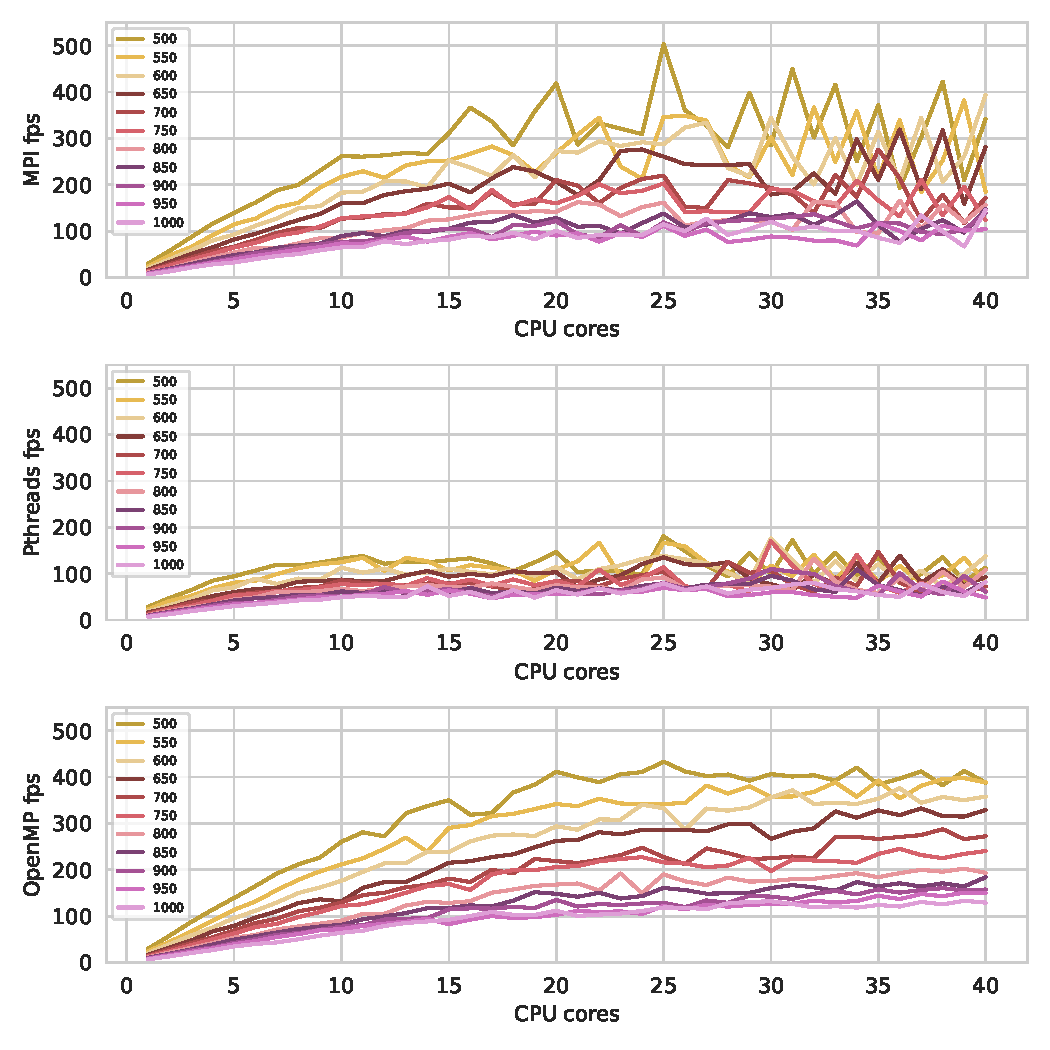
\includegraphics[width=\textwidth]{../analysis/fps-core-cpu.pdf}
    \caption{fps vs the number of threads/processes plot.}
    \label{fig:fps-core-cpu}
\end{figure}

\subsection{CPU parallelization}
From Figure \ref{fig:fps-core-cpu}, we can know that
when $n$ ranging from $500$ to $1000$,
MPI and OpenMP programs have similar performance when the number of processes/threads is under 20: 
fps steadily increases with threads/processes number while decreases with $n$.
The MPI program becomes quite unstable when the number of cores exceeds 20:
the reason might be the unstable communication traffic and CPU resources. 
Meanwhile, the Pthread program has low and relatively constant performance.
That may result from the Pthread function \lstinline|compute_pth| in
\lstinline|src/utils.h|.
In each iteration (each frame), the program will initialize \lstinline|nt|
threads, perform the computation parallelly and then merge these threads.
Different from OpenMP which is fully optimized, the initialization and
joining of threads in each iteration could be much more time-costly.
To fix this issue, one may initialize threads at the start of the program,
and join all threads after finishing all calculations.

The heatmap which indicate the rate of acceleration plotted in the Figure \ref{fig:heatmap-rate-cpu} 
provides some direct visualization of the performances of parallel variants.


\subsection{GPU parallelization}
GPU parallelization is much more massive than CPU parallelization.
This allows one to implemented $n>10^4$ with high fps, as Figure \ref{fig:fps-dim-gpu}
shows.
Notably, the gpu shared memory is used to accelerate the read operations.
(please refer to \lstinline|__shared| type and \lstinline|__syncthreads| function
in \lstinline|cudalib.cu|).
According to NVIDIA, the memory access on shared memory is
approximately 100$x$ faster than the global (\lstinline|__device__|) memory access.

\begin{figure}[t!]
    \centering
    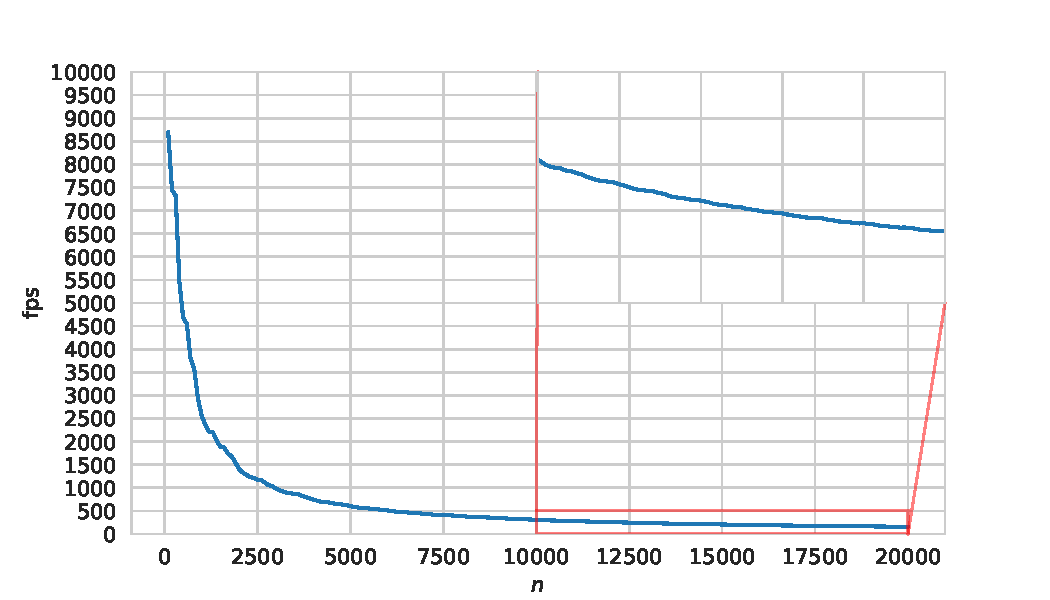
\includegraphics[width=\textwidth]{../analysis/fps-dim-gpu.pdf}
    \caption{CUDA fps vs $n$ plot.}
    \label{fig:fps-dim-gpu}
\end{figure}


\section{Conclusion}
In conclusion, four parallel computing schemes for $n$-body simulation 
are implemented and their performances are evaluated.
For large, ignoring the precision, one may use GPU to accelerate
the calculation.


\appendix
% \renewcommand\thefigure{\thesection.\arabic{figure}}
\counterwithin{figure}{section}

\newpage
\section{Supplementary figures}

\begin{figure}[h!]
    \centering
    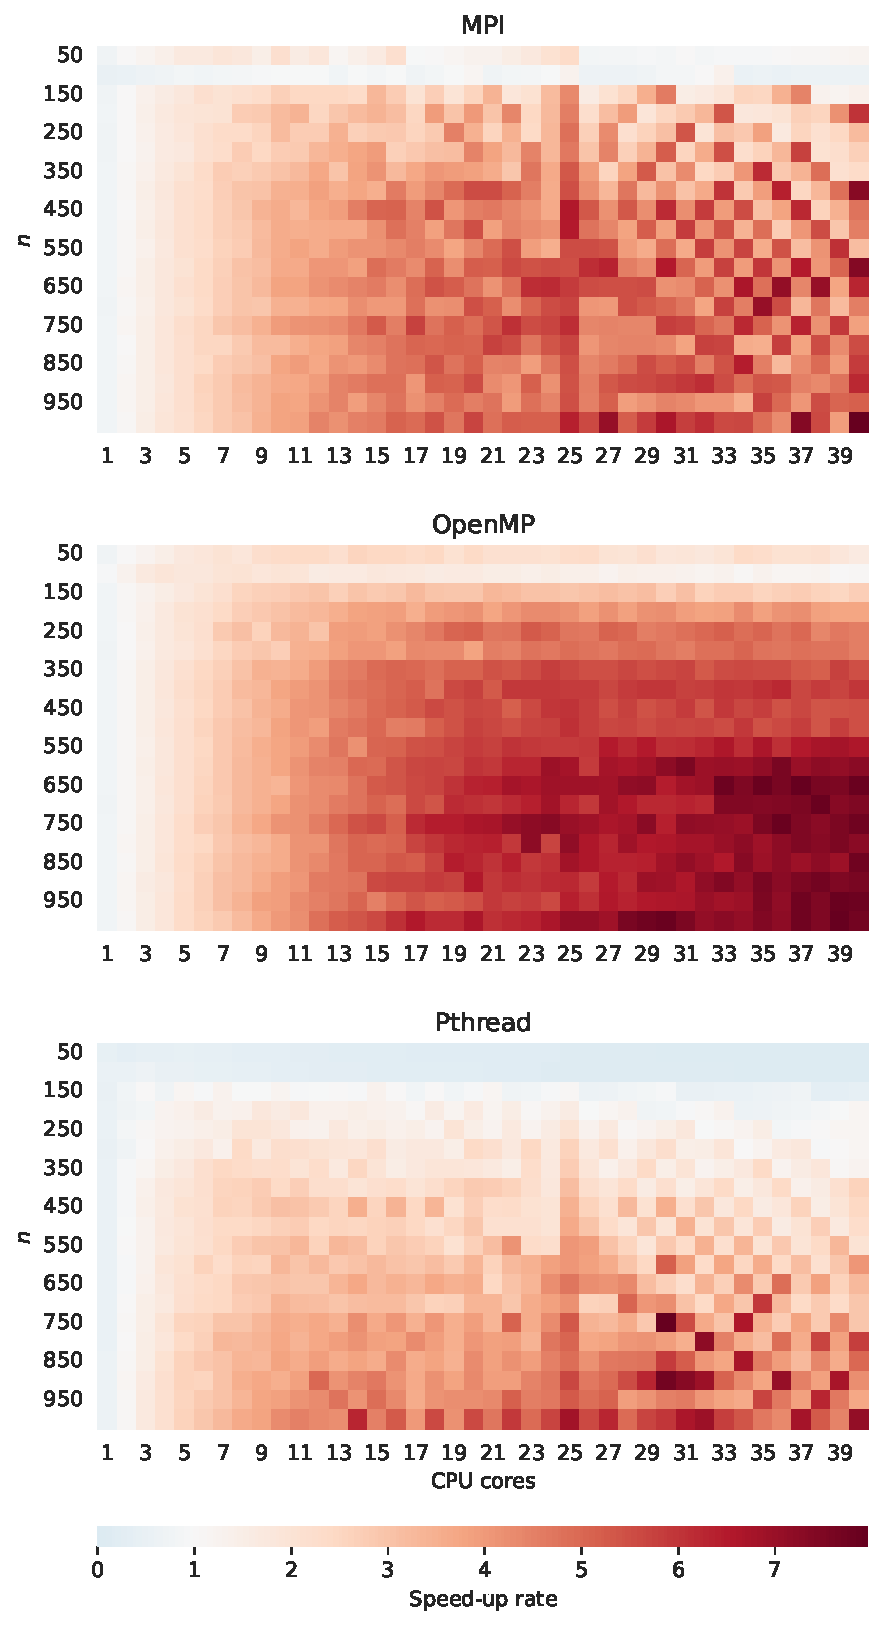
\includegraphics[width=0.66\textwidth]{../analysis/heatmap-rate-cpu.pdf}
    \caption{CUDA fps vs $n$ plot.}
    \label{fig:heatmap-rate-cpu}
\end{figure}

\clearpage
\newpage
\section{Source code}
\lstinputlisting[style=cpp,language=,title=\lstinline|CMakeLists.txt|]{../CMakeLists.txt}
\lstinputlisting[style=cpp,language=,title=\lstinline|src/CMakeLists.txt|]{../src/CMakeLists.txt}
\lstinputlisting[style=cpp,title=\lstinline|src/main.mpi.cpp|]{../src/main.mpi.cpp}
\lstinputlisting[style=cpp,title=\lstinline|src/utils.h|]{../src/utils.h}
\lstinputlisting[style=cpp,title=\lstinline|src/utils.cuh|]{../src/utils.cuh}
\lstinputlisting[style=cpp,title=\lstinline|src/const.h|]{../src/const.h}





% \end{multicols*}
\end{document}

